\documentclass[a4paper, 12pt]{article}
\usepackage[left=17mm, top=17mm, right=17mm, bottom=0mm, headsep=1em]{geometry} % лист а4, 12 кегль, тип документа - статья
\usepackage[utf8]{inputenc}  % кодировка вводимого текста
\usepackage[english, russian]{babel}  % подключение словарей с переносами англ и рус яз
\usepackage{amssymb, latexsym, amsmath, mathtext, bm, gensymb, amssymb}  % пакеты для работы с мат символами
\usepackage{indentfirst}  %  каждый абзац с красной строки
\setlength{\parindent}{4ex}
\linespread{0.4} % межстрочный интервал
 
\usepackage{graphicx}
\graphicspath{ {./images/} }
\usepackage{float}
\usepackage{wrapfig}

\usepackage{bm}
\usepackage{enumitem}
\usepackage[T2A]{fontenc}

\usepackage{fancyhdr}

\newcommand{\RNum}[1]{\uppercase\expandafter{\romannumeral #1\relax}}

\makeatletter
\AddEnumerateCounter{\asbuk}{\russian@alph}{щ}
\makeatother

\pagestyle{fancy}
\fancyhf{}
\rhead{Саженов Константин Станиславович}
\lhead{Группа М8О-108Б-19}
\chead{Вариант 22}
% \rfoot{Page \thepage}
\setlength{\headheight}{28pt}
% \set
\addtocounter{MaxMatrixCols}{3}

\newcommand{\Cmatrix}{
    \begin{pmatrix}
        -1 & 1 & 0 & 0 & 0 & 0 & 1 & 0 & 0 & 0 & 0 & 0 & 0 \\
        0 & 0 & 1 & 0 & 0 & 0 & 1 & 0 & 0 & 0 & 1 & 1 & 0 \\
        0 & 0 & 0 & 1 & -1 & 0 & 0 & 0 & -1 & 0 & 1 & 0 & 0 \\
        0 & 0 & 0 & 0 & 0 & -1 & 0 & 0 & 1 & 0 & 0 & 1 & 0 \\
        0 & 1 & 0 & 0 & 0 & 0 & 1 & -1 & 0 & 0 & 0 & 1 & 0 \\
        0 & 0 & 0 & 1 & 0 & 0 & 0 & 0 & 0 & 1 & 1 & 0 & 0 \\
        0 & 0 & 0 & 0 & 0 & 0 & 1 & 0 & 0 & 0 & 0 & 1 & 1
    \end{pmatrix}
}

\newcommand{\Bmat}{
    \begin{pmatrix}
        -1 & -1 &  0 &  0 &  0 &  0 &  0 & -1 &  0 &  0 &  0 &  0 &  0 \\
         0 &  1 &  1 &  0 &  0 &  0 & -1 &  0 &  0 &  0 &  0 &  0 & -1 \\
         1 &  0 &  0 &  0 &  0 & -1 &  1 &  0 &  0 &  0 &  0 & -1 &  0 \\
         0 &  0 &  0 &  0 &  0 &  0 &  0 &  1 & -1 &  1 & -1 &  1 & -1 \\
         0 &  0 & -1 & -1 &  0 &  0 &  0 &  0 &  0 &  0 &  1 &  0 &  0 \\
         0 &  0 &  0 &  0 & -1 &  1 &  0 &  0 &  1 &  0 &  0 &  0 &  0 \\ 
         0 &  0 &  0 &  1 &  1 &  0 &  0 &  0 &  0 & -1 &  0 &  0 &  0 
    \end{pmatrix}
}

\newcommand{\Uvector}{
    \begin{pmatrix}
        U_1 \\ \vdots \\ U_{13}
    \end{pmatrix}
}

\newcommand{\Ivector}{
    \begin{pmatrix}
        I_1 \\ \vdots \\ I_{13}
    \end{pmatrix}
}

\begin{document}
\section*{Задание \RNum{6}} 
\paragraph{Текст задания} Пусть каждому ребру неориентированного графа соответствует некоторый элемент
электрической цепи. Составить линейно независимые системы уравнений Кирхгофа для токов и
напряжений. Пусть первому и пятому ребру соответствуют источники тока с ЭДС
$E_1$ и $E_2$ (полярность выбирается произвольно), а остальные элементы являются сопротивлениями. Используя
закон Ома, и, предполагая внутренние сопротивления источников тока равными нулю, получить
систему уравнений для токов.

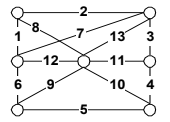
\includegraphics{6_chain}

\paragraph{Решение}
\begin{enumerate}
    \item Зададим произвольную ориентацию:
    \begin{figure}[h]
        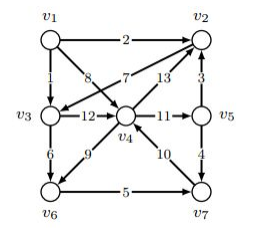
\includegraphics{6_orgraph}
    \end{figure}
    \item Построим произвольное остовное дерево:
    \begin{figure}[h]
        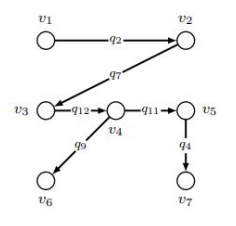
\includegraphics{6_tree}
    \end{figure}
    \begin{enumerate}[label*=\arabic*.]
        \item $ D_1 = (U_1, \emptyset) $
        \item $ D_2 = (\{U_{ 1}, U_{ 2}\}, \{U_{ 1}, U_{ 2}\})$
        \item $ D_3 = (\{U_{ 1}, U_{ 2}, U_{ 3}\}, \{U_{ 1}, U_{ 2}\}, \{U_{ 2}, U_{ 3}\})$
        \newpage
        \item $ D_4 = D_3 + \{U_{ 4}\} + \{U_{ 3}, U_{ 4}\} $
        \item $ D_5 = D_4 + \{U_{ 5}\} + \{U_{ 5}, U_{ 4}\} $
        \item $ D_6 = D_5 + \{U_{ 7}\} + \{U_{ 5}, U_{ 7}\} $
        \item $ D_7 = D_6 + \{U_{ 6}\} + \{U_{ 6}, U_{ 4}\} $
    \end{enumerate}
    \item Найдем базис циклов:
    \begin{enumerate}[label*=\arabic*.]
        \item 
        $(D + q_1) : \mu_1 : U_1 - U_2 - U_3 - U_1 \Rightarrow C(\mu_1) = 
            \begin{pmatrix}
            -1 & 1 & 0 & 0 & 0 & 0 & 1 & 0 & 0 & 0 & 0 & 0 & 0
            \end{pmatrix} 
        $
        \item 
        $(D + q_3) : \mu_2 : U_2 - U_3 - U_4 - U_5 - U_2 \Rightarrow C(\mu_2) = 
            \begin{pmatrix}
            0 & 0 & 1 & 0 & 0 & 0 & 1 & 0 & 0 & 0 & 1 & 1 & 0
            \end{pmatrix} 
        $
        \item 
        $(D + q_5) : \mu_3 : U_4 - U_5 - U_7 - U_6 - U_4 \Rightarrow C(\mu_3) = 
            \begin{pmatrix}
            0 & 0 & 0 & 1 & -1 & 0 & 0 & 0 & -1 & 0 & 1 & 0 & 0
            \end{pmatrix} 
        $
        \item 
        $(D + q_6) : \mu_4 : U_3 - U_4 - U_6 - U_3 \Rightarrow C(\mu_4) = 
            \begin{pmatrix}
            0 & 0 & 0 & 0 & 0 & -1 & 0 & 0 & 1 & 0 & 0 & 1 & 0
            \end{pmatrix} 
        $
        \item 
        $(D + q_8) : \mu_5 : U_1 - U_2 - U_3 - U_4 - U_1 \Rightarrow C(\mu_5) = 
            \begin{pmatrix}
            0 & 1 & 0 & 0 & 0 & 0 & 1 & -1 & 0 & 0 & 0 & 1 & 0
            \end{pmatrix} 
        $
        \item 
        $(D + q_{10}) : \mu_6 : U_4 - U_5 - U_7 - U_4 \Rightarrow C(\mu_6) = 
            \begin{pmatrix}
            0 & 0 & 0 & 1 & 0 & 0 & 0 & 0 & 0 & 1 & 1 & 0 & 0
            \end{pmatrix} 
        $
        \item 
        $(D + q_{13}) : \mu_7 : U_2 - U_3 - U_4 - U_2 \Rightarrow C(\mu_7) = 
            \begin{pmatrix}
            0 & 0 & 0 & 0 & 0 & 0 & 1 & 0 & 0 & 0 & 0 & 1 & 1
            \end{pmatrix} 
        $
        
    \end{enumerate}
    \item Цикломатическая матрица графа имеет вид:
    $$ C = \Cmatrix $$
    \item Выпишем закон Кирхгофа для напряжений: \\
    $ \Cmatrix \Uvector = 0 \Longleftrightarrow \left\{\begin{array}{lcl}
        -U_1 + U_2 + U_7 = 0\\
        U_3 + U_7 + U_{11} + U_{12} = 0 \\
        U_4 - U_5 - U_9 + U_{11} = 0 \\
        -U_6 + U_9 + U_{12} = 0 \\
        U_7 - U_8 + U_{12} = 0 \\
        U_4 + U_{10} + U_{11} = 0 \\
        U_7 + U_{12} + U_{13} = 0
    \end{array} \right. \Longrightarrow 
    \left\{ \begin{array}{lcl}
        U_1 = U_2 + U_7 \\ 
        U_3 = -U_7 - U_{11} - U_{12} \\ 
        U_5 = U_4 - U_9 + U_{11}\\ 
        U_6 = U_9 + U_{12}\\ 
        U_8 = U_7 + U_{12}\\
        U_{10} = -U_4 - U_{11}\\
        U_{13} = -U_7 - U_{12}
    \end{array}\right.$
    \item Найдем матрицу инцедентности $B$ орграфа:
    $$\begin{tabular}{ c| c| c |c| c| c| c| c|c| c |c |c |c |c |}
        & $q_1$ & $q_2$ & $q_3$ & $q_4$ & $q_5$ & $q_6$ & $q_7$ & $q_8$ & $q_9$ & $q_{10}$ & $q_{11}$ & $q_{12}$ & $q_{13}$\\ \hline
        $U_1$ & -1 & -1 &  0 &  0 &  0 &  0 &  0 & -1 &  0 &  0 &  0 &  0 &  0 \\ \hline
        $U_2$ &  0 &  1 &  1 &  0 &  0 &  0 & -1 &  0 &  0 &  0 &  0 &  0 & -1 \\ \hline
        $U_3$ &  1 &  0 &  0 &  0 &  0 & -1 &  1 &  0 &  0 &  0 &  0 & -1 &  0 \\ \hline
        $U_4$ &  0 &  0 &  0 &  0 &  0 &  0 &  0 &  1 & -1 &  1 & -1 &  1 & -1 \\ \hline
        $U_5$ &  0 &  0 & -1 & -1 &  0 &  0 &  0 &  0 &  0 &  0 &  1 &  0 &  0 \\ \hline
        $U_6$ &  0 &  0 &  0 &  0 & -1 &  1 &  0 &  0 &  1 &  0 &  0 &  0 &  0 \\ \hline
        $U_7$ &  0 &  0 &  0 &  1 &  1 &  0 &  0 &  0 &  0 & -1 &  0 &  0 &  0 \\ \hline
        \end{tabular}
        $$
        $$ B = \Bmat $$
    \newpage
    \item Выпишем уравнения Кирхгофа для токов:
    $$ \Bmat \cdot \Ivector = 0 \Rightarrow $$
    \begin{align}\left\{ \begin{array}{lcr}
        I_1 + I_2 + I_8 = 0 \\
        I_2 + I_3 - I_7 + I_{13} = 0 \\
        I_1 - I_6 + I_7 - I_{12} = 0 \\
        I_{11} - I_3 - I_4 = 0 \\
        I_{7} - I_6 + I_9 = 0 \\
        I_{5} + I_6 - I_{10} = 0 
    \end{array} \right. \end{align}
    \item Подставим закон Ома:
    \begin{align}
        \left\{ \begin{array}{lcr}
            E_1 = I_2 R_2 + I_7 R_7 \\
            E_2 = I_4 R_4 - I_9 R_9 + I_{11} R_{11} \\
            I_3 R_3 + I_7 R_7 + I_{11} R_{11} + I_{12} R_{12} = 0 \\
            I_6 R_6 - I_9 R_9 - I_{12} R_{12} = 0 \\
            I_8 R_8 - I_7 R_7 - I_{12} R_{12} = 0 \\
            I_{10} R_{10} + I_4 R_4 + I_{11} R_{11} = 0 \\
            I_{13} R_{13} I_7 R_7 + I_{12} R_{12} = 0
        \end{array}\right.
    \end{align}
    \item Совместная система состоит из систем (1) и (2). 13 уравнений и 13 неизвестных -- 
    токи $ I_1 \dots I_{13} ;$ ЭДС $ E_1, E_2$ Сопротивления $R_2 ; R_3 ; R_4 ; R_5 ; R_6 ; R_7 ; R_8 ; R_9 ; R_{10} ; R_{11} ; R_{12} ; R_{13}$ - известны
\end{enumerate}

\end{document}